% \documentclass[svgnames]{article}
% To make png: pdftopng -r 900 -alpha LucasBoston.pdf temp.png
\documentclass[svgnames,convert={density=900,size=720x600,outext=.png}]{standalone}
\usepackage{tikz}
\usetikzlibrary{calc,trees,positioning,arrows,chains,shapes.geometric,backgrounds,
  decorations.pathreplacing,decorations.pathmorphing,shapes,snakes,automata,
  matrix,shapes.symbols,mindmap,shadows,petri}
% \renewcommand{\rmdefault}{phv} % Arial
% \renewcommand{\sfdefault}{phv} % Arial
% \usepackage{amsmath} % to allow Sans font in math


\begin{document}
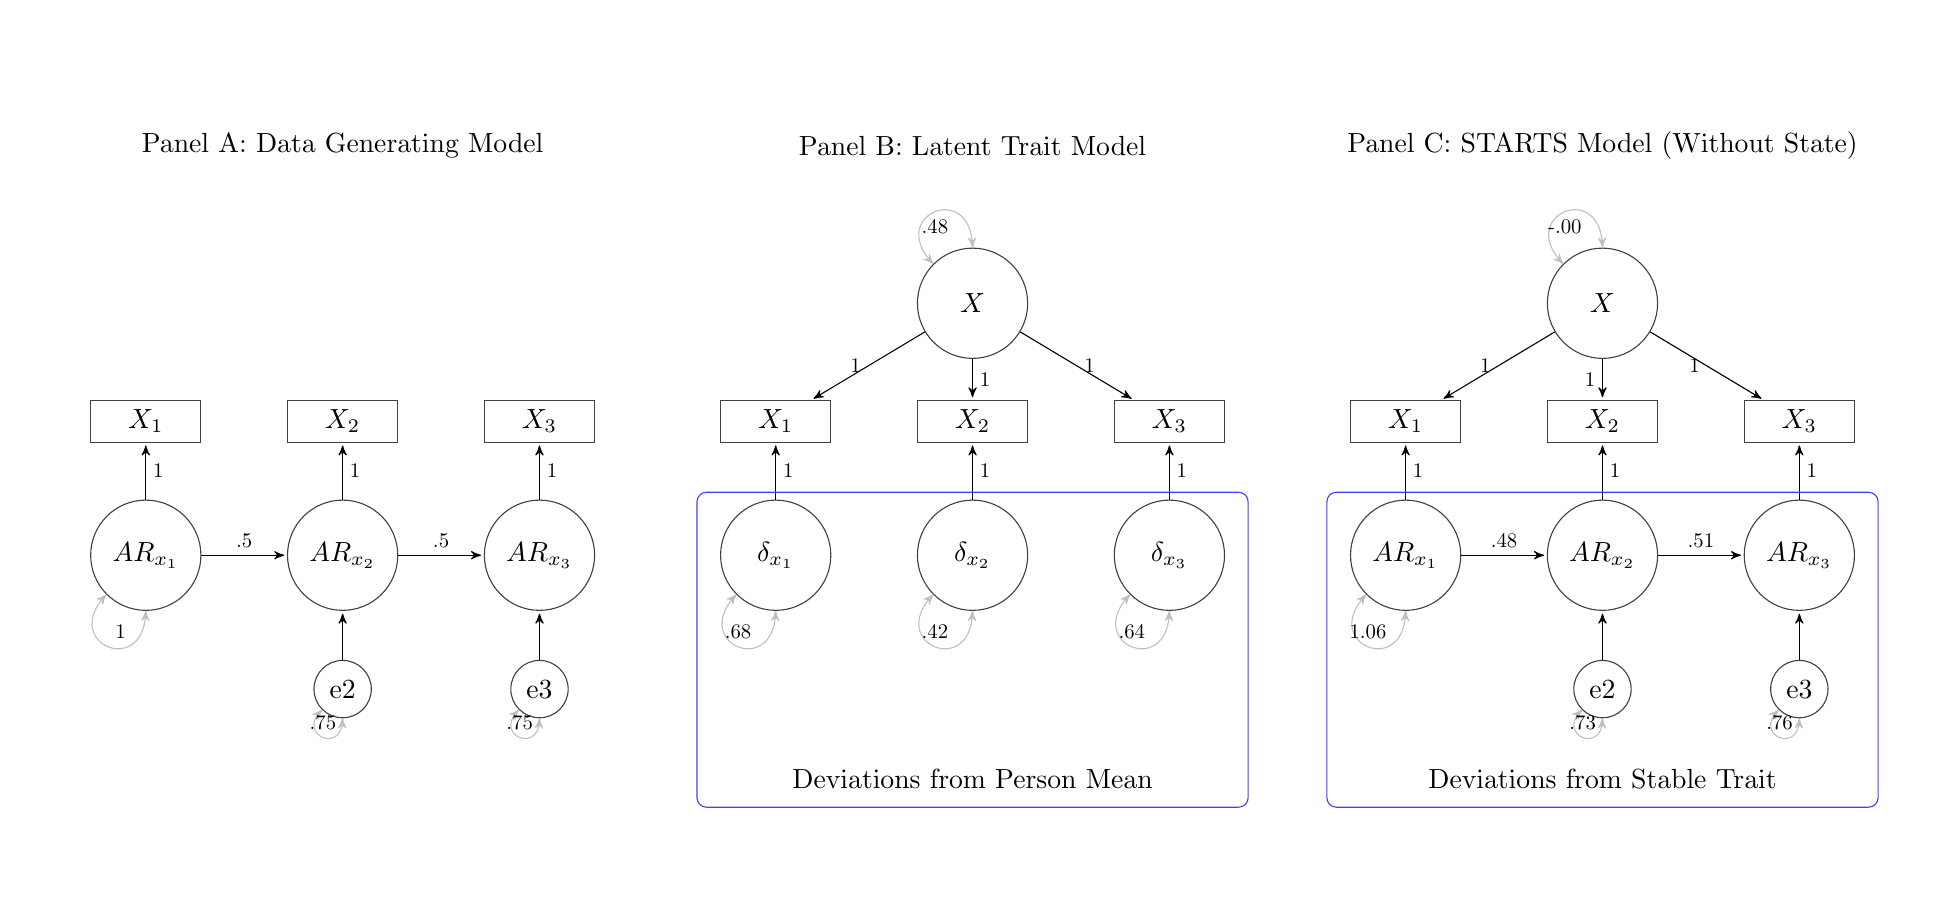
\begin{tikzpicture}[node distance=2.5cm,>=stealth',bend angle=45,auto]
  \useasboundingbox (-1.5,-6) rectangle (22.5,5);
  \tikzset{
    latentTrait/.style={circle,draw=black!75,minimum size=14mm,, align=center},
    latentAR/.style={circle,draw=black!75,minimum size=14mm},
    observed/.style={rectangle,draw=black!75,minimum width=14mm, align=center},
    error/.style={circle,draw=black!75,minimum size=.9mm},
    errorAR/.style={circle,draw=black!75,minimum size=1mm, node distance=1.7cm},
    state/.style={circle,draw=black!75,minimum size=1mm, scale=.75, align=center, node distance=1.7cm},
    hspace/.style={node distance=2.7cm},
    vspace/.style={node distance=4.25cm},
    % edge styles
    indicatorDist/.style={node distance=1.7cm},
    errorDist/.style={node distance=.73cm},
    newARDist/.style={node distance=1.2cm},
    stabDist/.style={node distance=1cm},
    variance/.style={<->, bend left=250, looseness=4, draw=lightgray},
    %label styles
    constraints/.style={scale=.75,above},
    constraintsb/.style={scale=.75,below},
    constraintsl/.style={scale=.75,left},
    constraintsr/.style={scale=.75,right},
    %
    backBox/.style={rectangle,draw=blue!75,rounded corners=.8ex,minimum width=11cm,minimum height=2.8cm}
    
  }

  %% Data-Generating Model
  \node [observed] (xt1) {$X_1$};
  \node [latentAR, indicatorDist] (ar1) [below of=xt1] {$AR_{x_1}$}
  edge [post] node[constraintsr] {1} (xt1);

  \draw [variance] (ar1.south west) to node[above right, scale=.75] {1} (ar1.south);

  \node [observed] (xt2) [right of=xt1] {$X_2$};
  \node [latentAR, indicatorDist] (ar2) [below of=xt2]  {$AR_{x_2}$}
  edge [post] node[constraintsr] {1} (xt2)
  edge [pre] node[constraints] {.5} (ar1);

  \node [observed] (xt3) [right of=xt2] {$X_3$};
  \node [latentAR, indicatorDist] (ar3) [below of=xt3]  {$AR_{x_3}$}
  edge [post] node[constraintsr] {1} (xt3)
  edge [pre] node[constraints] {.5} (ar2);
  \node (label1) [above of=xt2, node distance=3.5cm] {Panel A: Data Generating Model};

  \node [errorAR] (ar2e) [below of=ar2] {e2} edge [post] (ar2);
  \draw [variance] (ar2e.south west) to node[scale=.75, above] {.75} (ar2e.south);    
  \node [errorAR] (ar3e) [below of=ar3] {e3} edge [post] (ar3);
  \draw [variance] (ar3e.south west) to node[scale=.75, above] {.75} (ar3e.south);    





  
  %% Person-Means
  \node [observed, node distance=3cm] (m2xt1) [right of=xt3] {$X_1$};
  \node [latentAR, indicatorDist] (m2ar1) [below of=m2xt1] {$\delta_{x_1}$}
  edge [post] node[constraintsr] {1} (m2xt1);
  
  \draw [variance] (m2ar1.south west) to node[constraints] {.68} (m2ar1.south);

  \node [observed] (m2xt2) [right of=m2xt1] {$X_2$};
  \node [latentAR, indicatorDist] (m2ar2) [below of=m2xt2]  {$\delta_{x_2}$}
  edge [post] node[constraintsr] {1} (m2xt2);

  \draw [variance] (m2ar2.south west) to node[constraints] {.42} (m2ar2.south);

  \node [observed] (m2xt3) [right of=m2xt2] {$X_3$};
  \node [latentAR, indicatorDist] (m2ar3) [below of=m2xt3]  {$\delta_{x_3}$}
  edge [post] node[constraintsr] {1} (m2xt3);

  \draw [variance] (m2ar3.south west) to node[constraints] {.64} (m2ar3.south);

  \node [latentTrait] (st) [above of=m2xt2, node distance=1.5cm] {$X$}
  edge [post] node[constraintsl] {1} (m2xt1) 
  edge [post] node[constraintsr] {1} (m2xt2)
  edge [post] node[constraintsr] {1} (m2xt3);

  \draw [variance] (st.north) to node[scale=.75, below] {.48} (st.north west);  

  \node [rectangle, node distance=2.9cm, draw=blue!75, rounded corners=.8ex,
  minimum width=7cm, minimum height=4cm, label={[yshift=-3.9cm] Deviations from Person Mean}] (deviations) [below of=m2xt2] {};

  \node (label2) [above of=m2xt2, node distance=3.5cm] {Panel B: Latent Trait Model};
  


  %% RI-CLPM
  \node [observed, node distance=3cm] (m3xt1) [right of=m2xt3] {$X_1$};
  \node [latentAR, indicatorDist] (m3ar1) [below of=m3xt1] {$AR_{x_1}$}
  edge [post] node[constraintsr] {1} (m3xt1);

  \draw [variance] (m3ar1.south west) to node[constraints] {1.06} (m3ar1.south);

  \node [observed] (m3xt2) [right of=m3xt1] {$X_2$};
  \node [latentAR, indicatorDist] (m3ar2) [below of=m3xt2]  {$AR_{x_2}$}
  edge [post] node[constraintsr] {1} (m3xt2)
  edge [pre] node[constraints] {.48} (m3ar1);

  \node [observed] (m3xt3) [right of=m3xt2] {$X_3$};
  \node [latentAR, indicatorDist] (m3ar3) [below of=m3xt3]  {$AR_{x_3}$}
  edge [post] node[constraintsr] {1} (m3xt3)
  edge [pre] node[constraints] {.51} (m3ar2);

  \node [latentTrait] (st3) [above of=m3xt2, node distance=1.5cm] {$X$}
  edge [post] node[constraintsl] {1} (m3xt1)
  edge [post] node[constraintsl] {1} (m3xt2)
  edge [post] node[constraintsl] {1} (m3xt3);

  \draw [variance] (st3.north) to node[scale=.75, below] {-.00} (st3.north west);  

  \node [errorAR] (m3ar2e) [below of=m3ar2] {e2} edge [post] (m3ar2);
  \draw [variance] (m3ar2e.south west) to node[scale=.75, above] {.73} (m3ar2e.south);  
  \node [errorAR] (m3ar3e) [below of=m3ar3] {e3} edge [post] (m3ar3);
  \draw [variance] (m3ar3e.south west) to node[scale=.75, above] {.76} (m3ar3e.south);    
  
  \node [rectangle, node distance=2.9cm, draw=blue!75, rounded corners=.8ex,
  minimum width=7cm, minimum height=4cm, label={[yshift=-3.9cm] Deviations from Stable Trait}] (m3deviations) [below of=m3xt2] {};

  \node (label3) [above of=m3xt2, node distance=3.5cm] {Panel C: STARTS Model (Without State)};
  

  


\end{tikzpicture}
\end{document}